\documentclass{article}

\title{ARI3129 Generative AI Usage Journal}
\author{Daniel Pace, Amy Spiteri, Ellyn Rose Debrincat, Joachim Grech}
\date{\today}

\usepackage[utf8]{inputenc}
\usepackage[margin=1in]{geometry}
\usepackage{graphicx}
\usepackage{hyperref}
\usepackage{ragged2e}
\usepackage{listings}
\usepackage{xcolor}
\usepackage{subcaption}

\lstdefinestyle{py}{
    basicstyle=\ttfamily\small,                 % Use a monospaced font
    keywordstyle=\color{purple},                % Keywords in purple
    stringstyle=\color{blue},                   % Strings in blue
    commentstyle=\color{green!60!black},        % Comments in green
    numbers=left,                               % Line numbers on the left
    numberstyle=\tiny\color{gray},              % Line number style
    stepnumber=1,                               % Line number step
    showstringspaces=false,                     % Do not show spaces in strings
    breaklines=true,                            % Allow line breaking
    tabsize=4,                                  % Set tab size
    language=Python,                            % Set the language for syntax highlighting
    numbersep=4pt,                              % Reduce the distance between line numbers and code (default is 10pt)
    belowskip=1.5em
}
\setlength{\parindent}{0pt}
\hyphenpenalty=10000
\exhyphenpenalty=10000
\sloppy

\renewcommand{\refname}{\vspace{-1.5em}}

\begin{document}

\pagenumbering{roman}

\begin{titlepage}
    \centering
    \vspace*{2cm}
    {
\includegraphics[scale=0.5]{umcrest.jpg}\\[2em]}
    {\Huge\bfseries Computer Vision Group Project\\[0.5cm]}
    {\Large ARI3129\\[0.5cm]}
    {\Large Generative AI Usage Journal\\[0.5cm]}
    {\large Daniel Pace, Amy Spiteri, Ellyn Rose Debrincat, Joachim Grech\\[0.5cm]}
    {\large \today}
\end{titlepage}

\tableofcontents
\newpage
\pagenumbering{arabic}
\justifying\noindent

\section{Introduction}
% Briefly describe the generative AI models you chose to use and the rationale behind that choice. (Maximum of 1 page)
Generative AI tools were used in this assignment. The models used include:
\begin{itemize}
    \item Gemini 3 Pro: Chosen for its advanced thinking capabilities and large context window, making it suitable for complex problem-solving tasks. Also selected thanks to the free subscription provided by the University.
    \item Claude Sonnet 4.5: Selected for its high performance in coding tasks and problem-solving. The more formal tone it tends to use was also found to be beneficial for academic purposes.
    \item ChatGPT 5.2: Selected for its versatility in generating diverse solutions and quick troubleshooting.
    \item Antigravity: Utilized as an agentic AI assistant to streamline the development process, automate repetitive tasks, and perform precise error detection across the codebase and documentation.
    \item NotebookLM: Chosen for its ability to generate information from specific sources, summarize complex materials, and help structure research findings in a clear, organized way.
\end{itemize}

\section{Ethical Considerations}

The integration of generative AI tools into academic research raises several ethical considerations that warrant careful examination and mitigation strategies.

\subsubsection*{Data Bias and Model Limitations}

Generative AI models reflect biases inherent in their training data, which can manifest in code suggestions favouring certain programming paradigms or in technical explanations using biased terminology. To mitigate these concerns, we adopted a critical evaluation approach where all AI-generated content was reviewed and verified against authoritative sources such as official documentation and peer-reviewed papers. AI outputs were treated as starting points for investigation rather than definitive answers.

\subsubsection*{Privacy and Data Security}

Privacy considerations were paramount in our AI usage. We ensured that no sensitive information from our dataset was shared with AI platforms. All interactions were limited to general technical queries and code debugging that did not expose proprietary project details. We remained mindful of data retention policies, recognizing that prompts may be stored and used for model training.

\section{Methodology}
% Outline the methods and steps to integrate the generative AI model into your work. Which tools did you use, and in which sequence? Did you create your own pipeline, or did you use a single tool? There is no wrong answer, and this journal aims for transparency and accountability.
The use of generative AI in our project can be classified into the following two main categories:
\subsubsection*{Automatic, in-line code suggestions}
In Visual Studio Code, the copilot extension was used to provide real-time code suggestions and completions. This tool was primarily employed during coding sessions to enhance productivity and reduce syntax errors. The AI model provided context-aware suggestions based on the current codebase, which were then reviewed and integrated by the team members. The free student subscription provided by GitHub was utilized for this purpose, giving us access to premium models and features.

\subsubsection*{Prompt-Response interactions for specific tasks}
For other tasks, such as debugging certain issues, or generating documentation outlines, we used web-based interfaces for Gemini 3 Pro, Claude Sonnet 4.5, and ChatGPT 5.2. The process involved formulating specific prompts related to the task at hand, submitting them to the AI model, and then evaluating the generated responses. The outputs were critically assessed for accuracy and relevance before being incorporated into our project workflow.

\section{Prompts and Responses}
% List down the specific prompts that were used with the generative AI model and that you found noteworthy. For each prompt, also include the generated response and explain how it contributed to improving your project. It is advisable to use screenshots for this part.
The following are examples of noteworthy prompts and their outputs that highlight how the tools were used in this project.

\subsubsection*{Creating to-do lists for project management}
Before starting the project, a checklist was created to outline the steps needed to complete the assignment, as shown in Figure~\ref{fig:checklist}. This checklist allowed us to break down the project into manageable tasks and ensured that we stayed on track throughout the development process.

\begin{figure}[htbp]
    \centering
    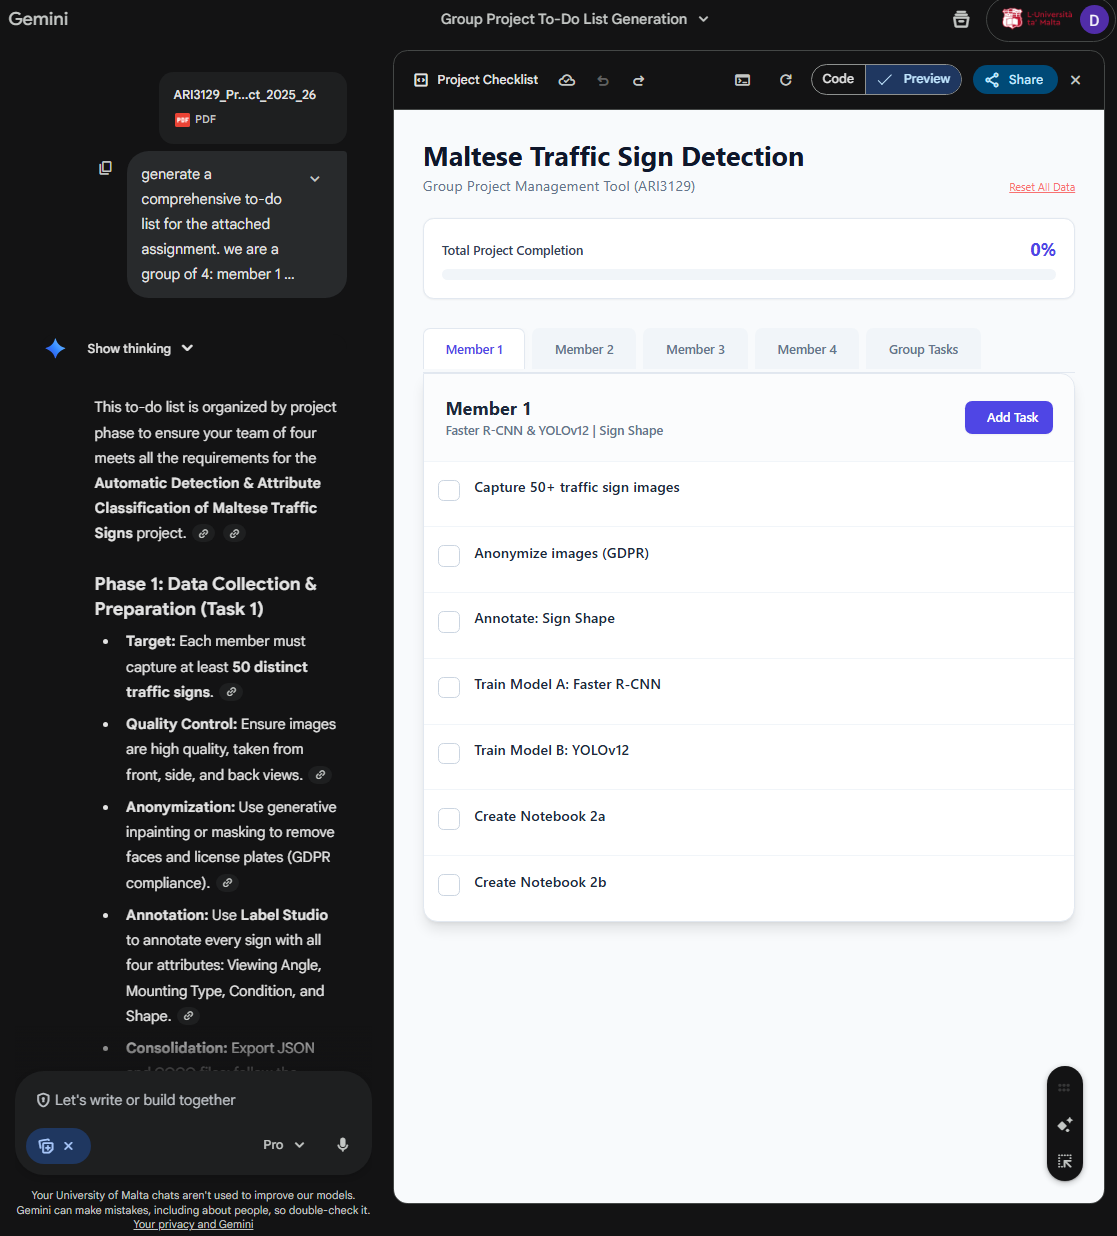
\includegraphics[width=0.7\textwidth]{checklist.png}
    \caption{Prompt: Creating a project to-do list}\label{fig:checklist}
\end{figure}

Notably, the checklist html generated by the AI model was fully functional and would remember any modifications made to it, allowing us to track our own progress effectively. Some limitations were observed, such as the inability to automatically sync the progress of the other members, as well as the contents of the checklist itself not being entirely accurate. The first issue was ignored as it was not worth the effort to implement a more complex solution, while the second issue was resolved by manually editing the checklist to better reflect our project requirements. 

The generation of the checklist in Figure~\ref{fig:checklist} was done using 2 prompts, one to generate the initial list of tasks, and another to convert it into an interactive html format.

\subsubsection*{Generating report outlines}
These 2 prompts (Figure~\ref{fig:chatlogs_1_2}) illustrate how generative AI was used to structure the report, in accordance with the provided guidelines.

\begin{figure}[htbp]
    \centering
    \begin{subfigure}[b]{0.45\textwidth}
        \centering
        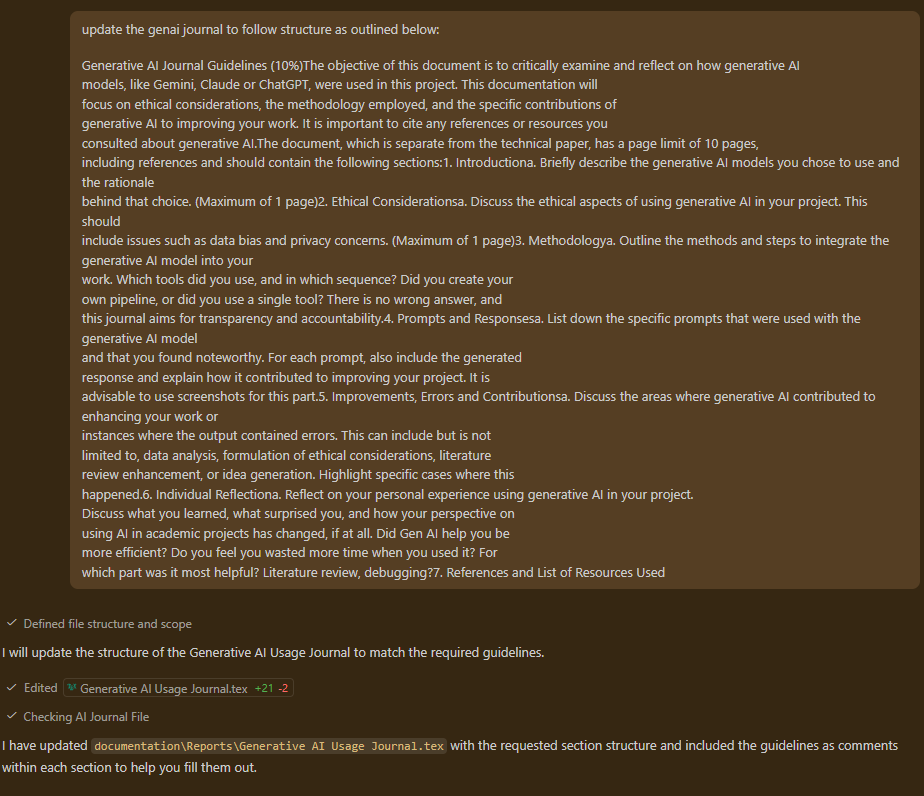
\includegraphics[width=\textwidth]{chatlog_1.png}
        \caption{Prompt 1: Generating report outline}\label{fig:chatlog_1}
    \end{subfigure}
    \hfill
    \begin{subfigure}[b]{0.45\textwidth}
        \centering
        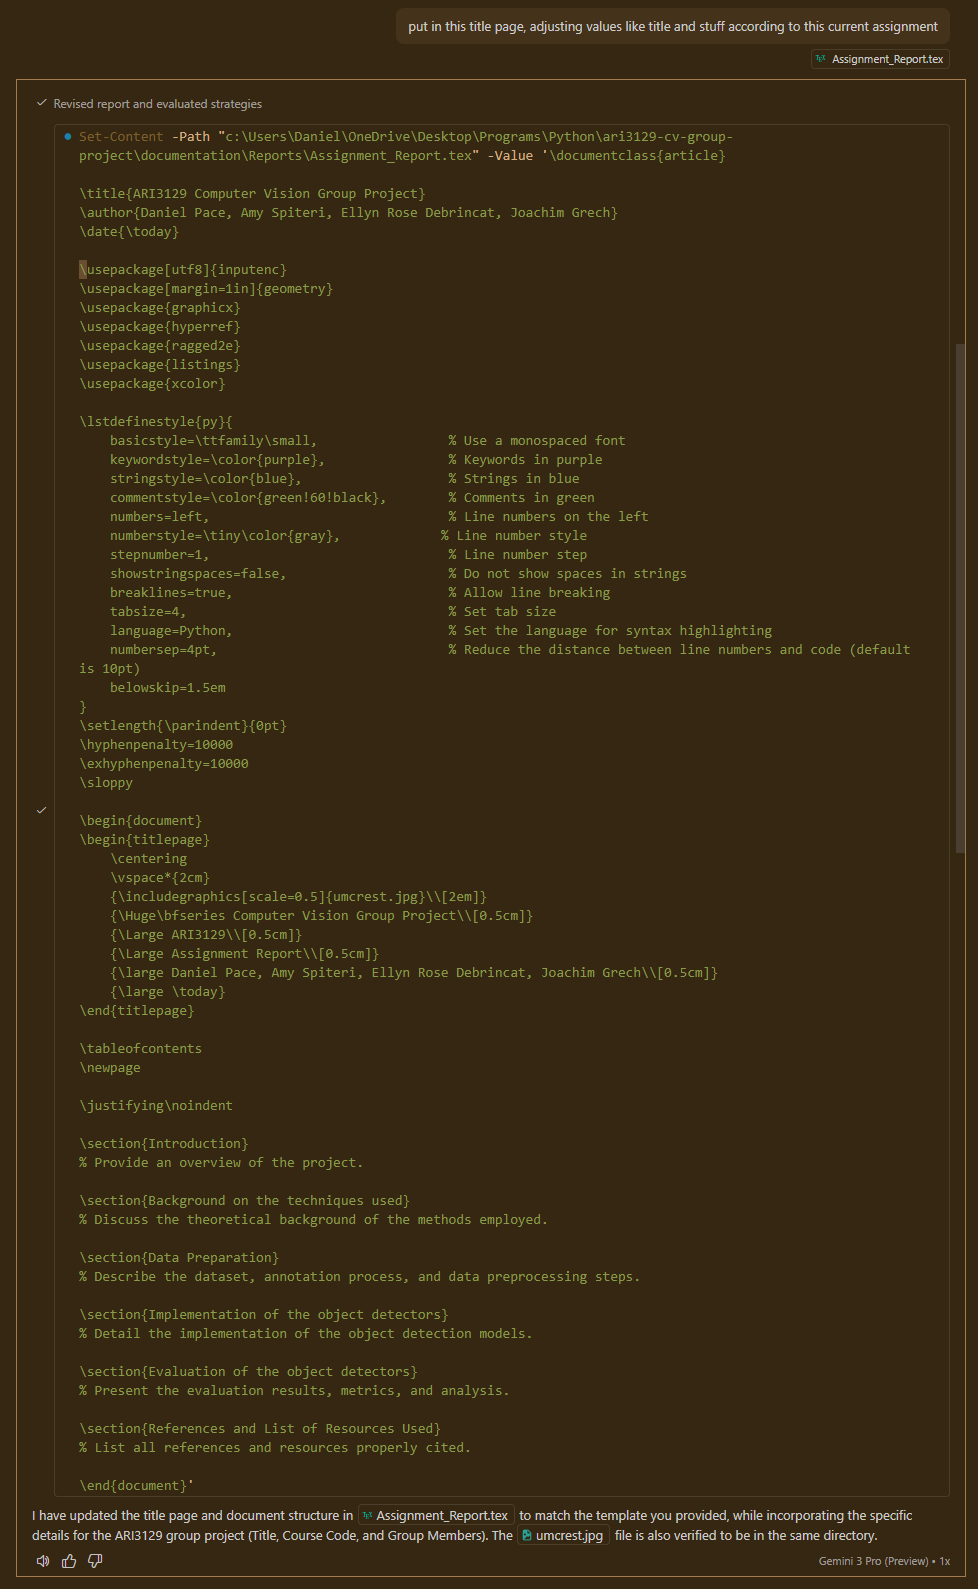
\includegraphics[width=\textwidth]{chatlog_2.png}
        \caption{Prompt 2: Creating title page}\label{fig:chatlog_2}
    \end{subfigure}
    \caption{Prompts used to generate report structure}\label{fig:chatlogs_1_2}
\end{figure}

After the initial outputs were generated, we modified the structure slightly to better fit our specific project needs. The AI-generated outlines provided a solid foundation, which we then customized to ensure clarity and coherence in our report.

\subsubsection*{Debugging and fixing errors}

Generative AI tools were also used to help with understanding and debugging errors in our code in an efficient way, as can be seen in Figure~\ref{fig:debugging}. Using these tools for help in fixing errors was useful as they gave us a way to quickly understand the main issue behind what was causing the problems, as well as suggesting ways on how to fix them. Using Generative AI as a coding assistant in this way helped save a lot of time that otherwise would be spent trying to debug confusing errors.

\begin{figure}[htbp]
    \centering
    \begin{subfigure}[b]{0.45\textwidth}
        \centering
        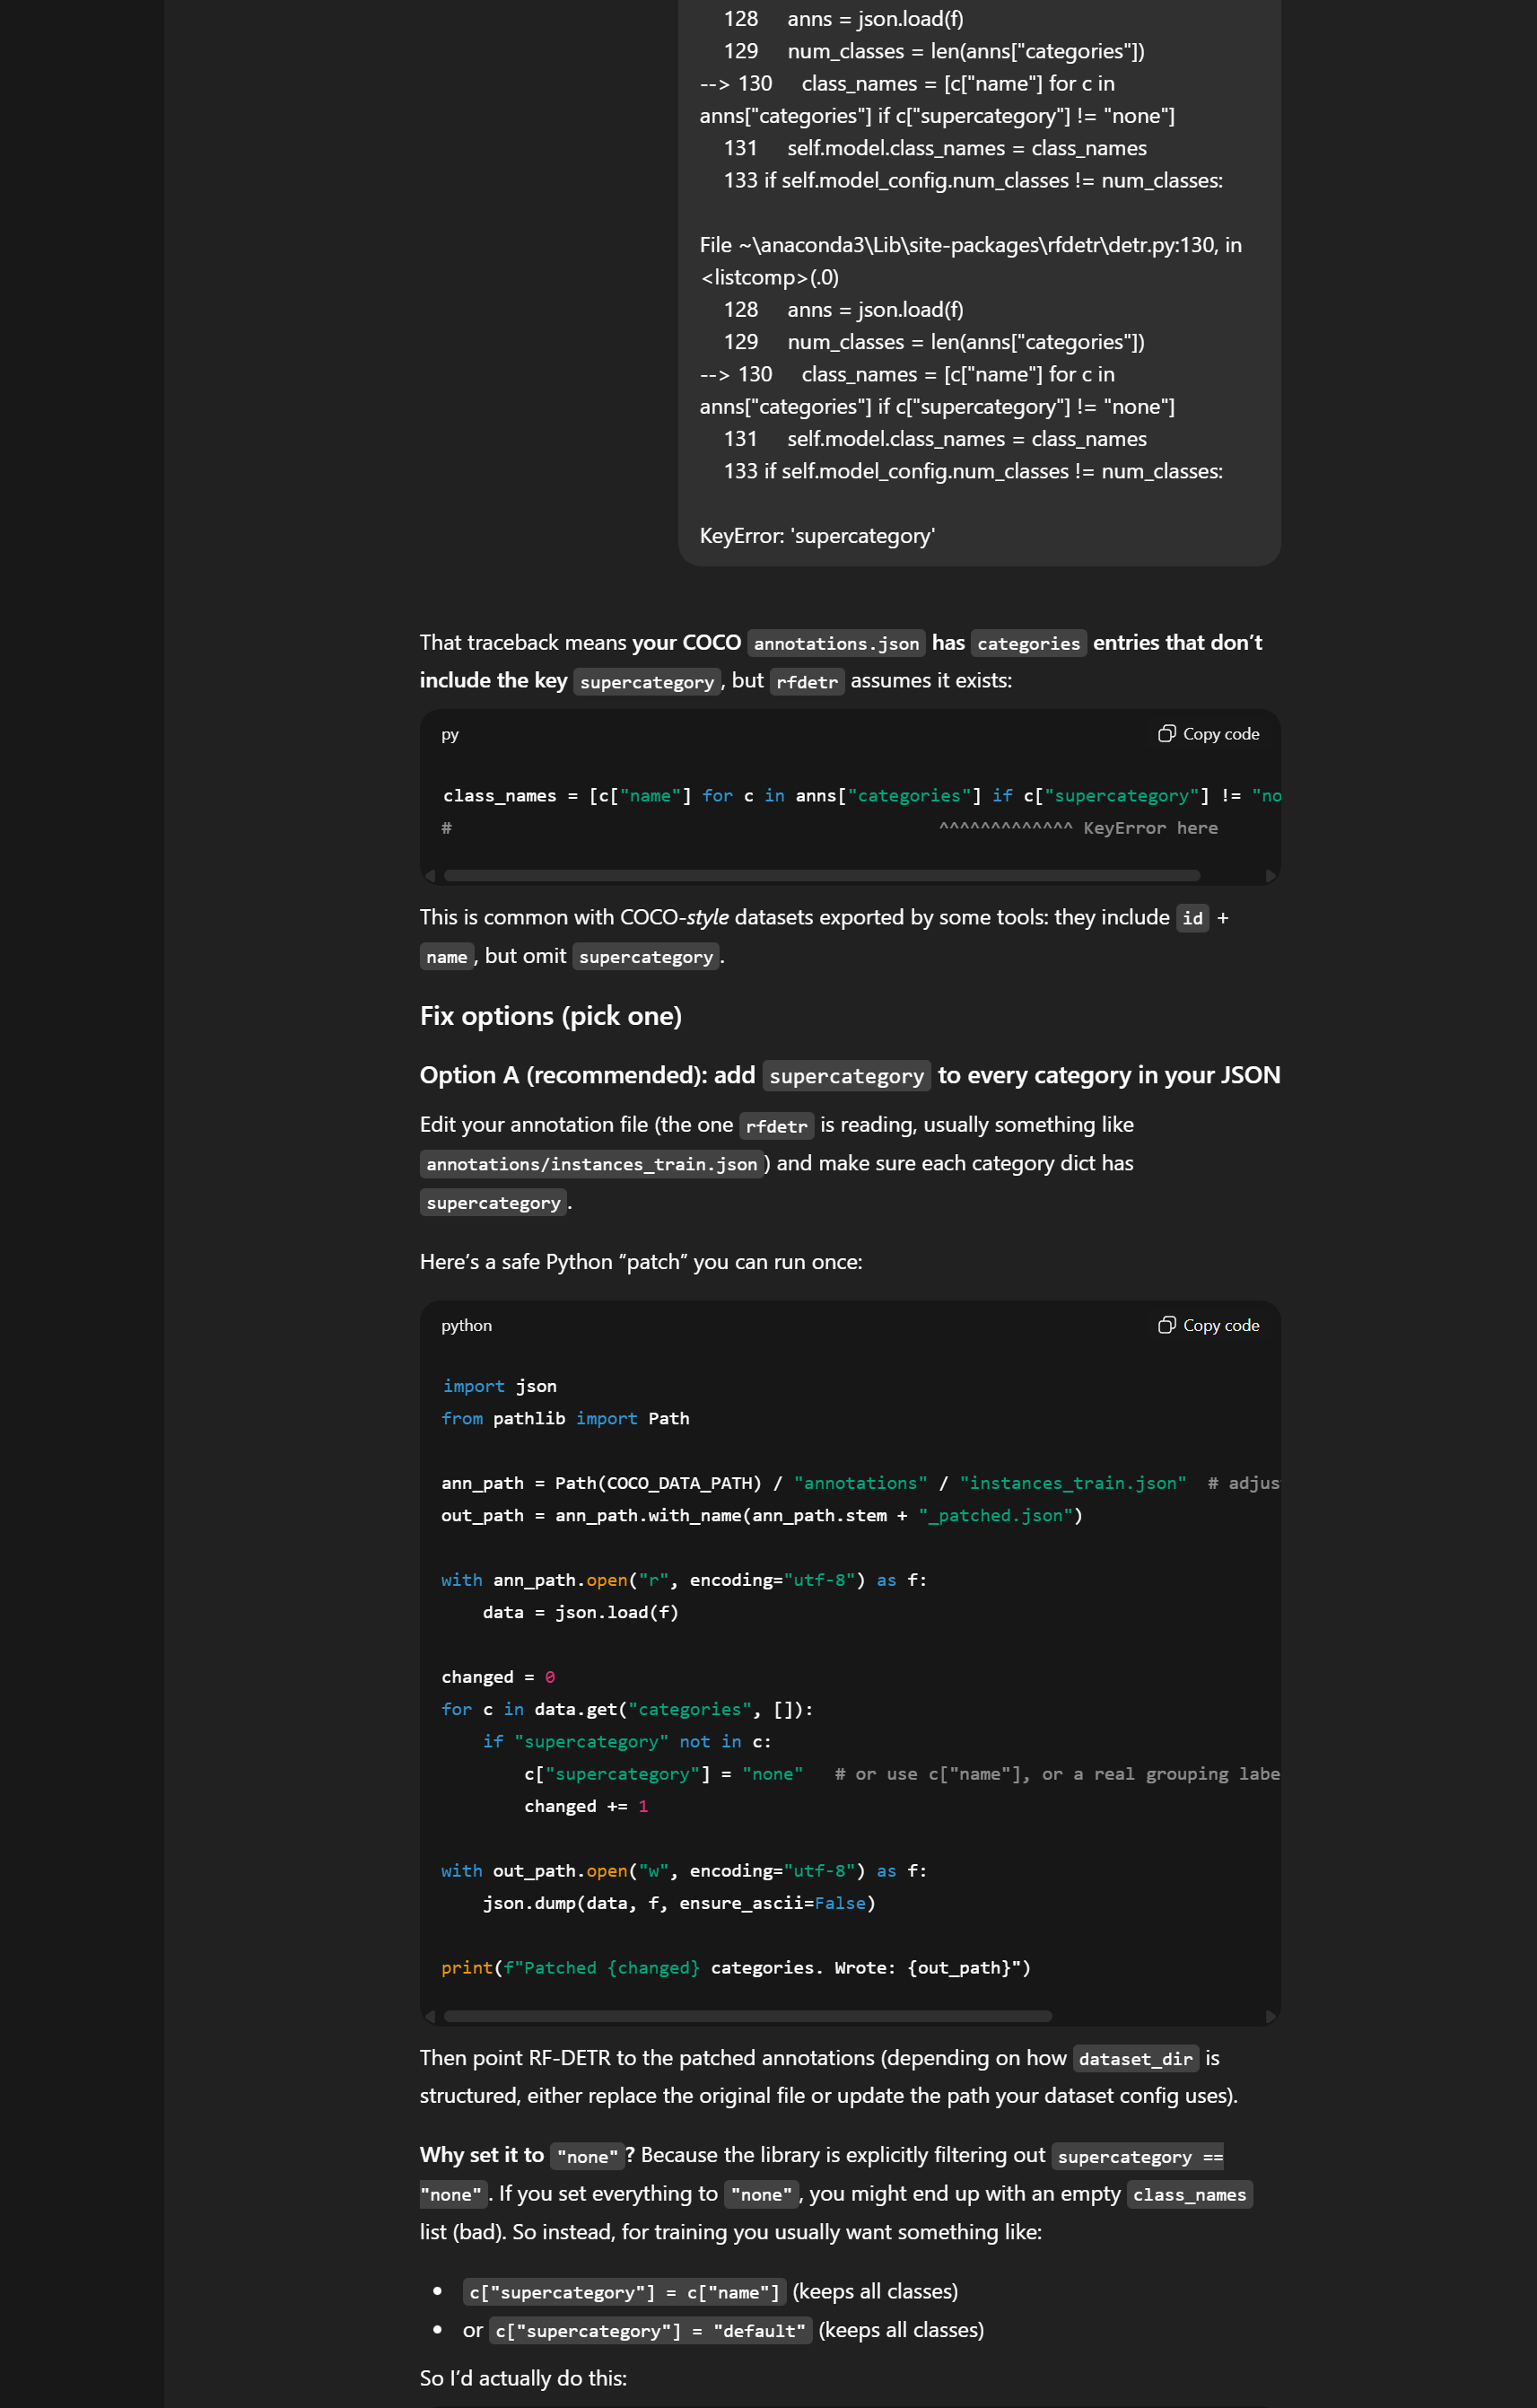
\includegraphics[width=\textwidth]{debugging1.png}
    \end{subfigure}
    \hfill
    \begin{subfigure}[b]{0.45\textwidth}
        \centering
        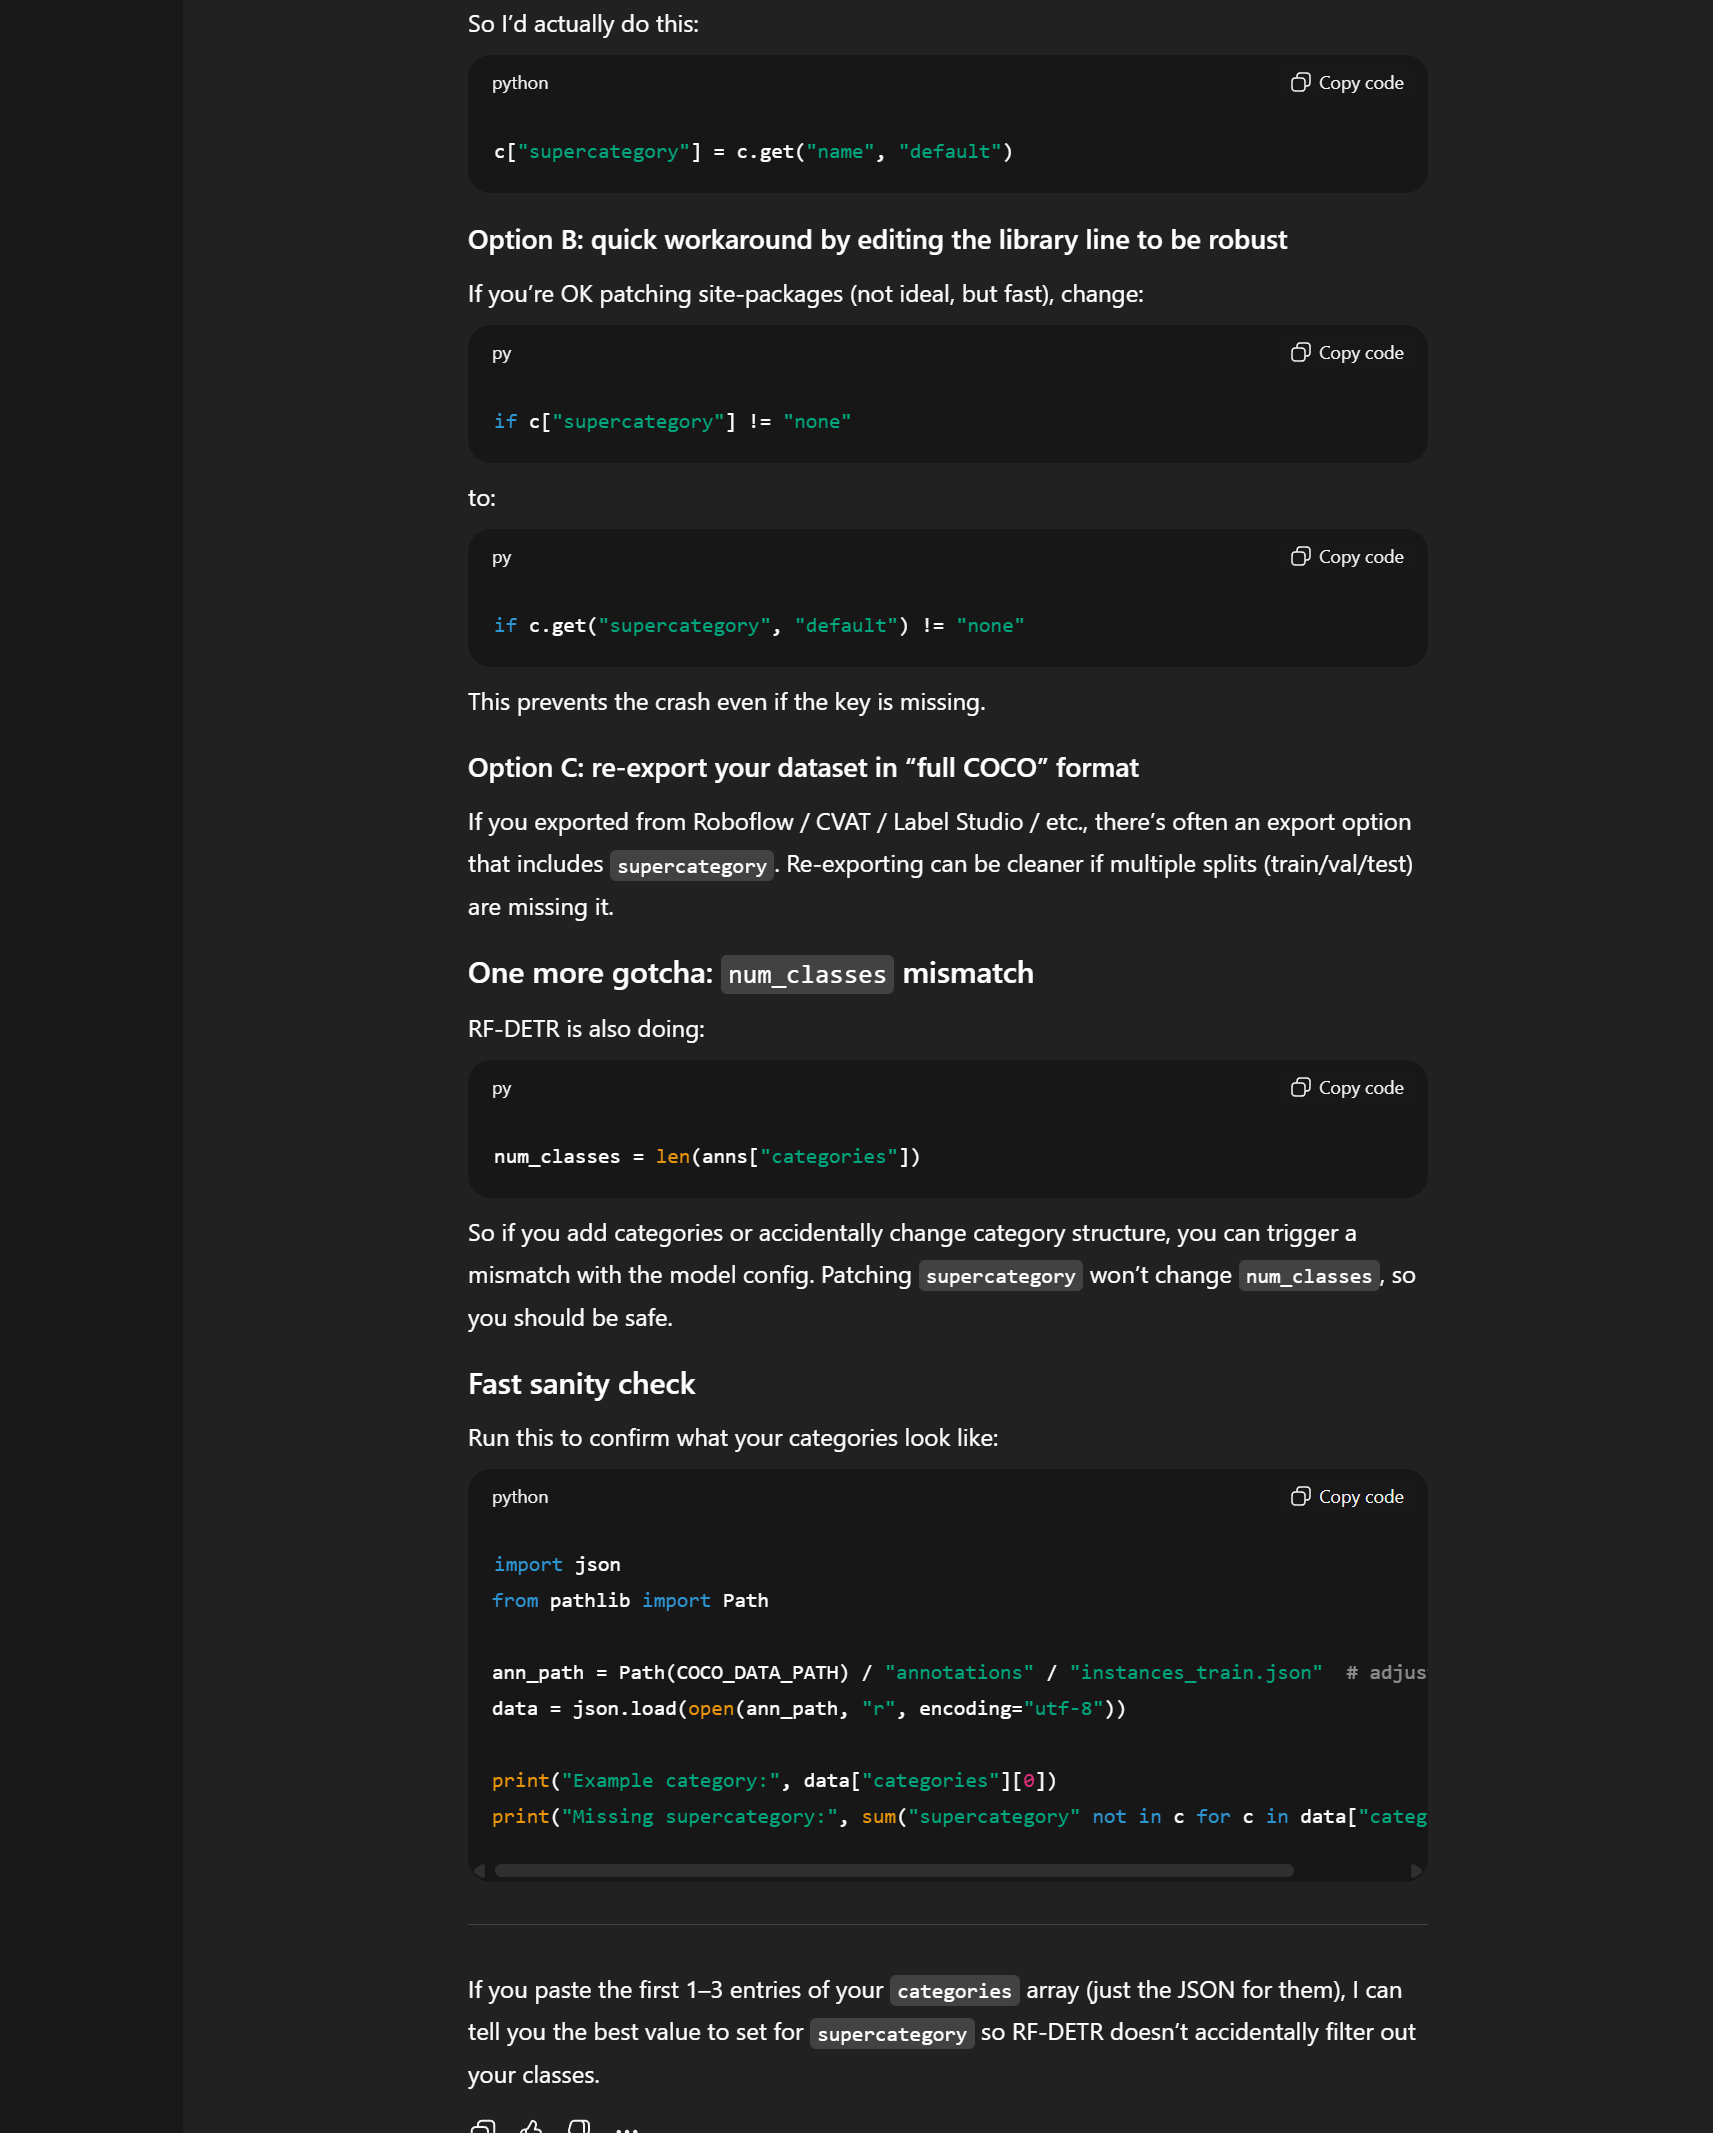
\includegraphics[width=\textwidth]{debugging2.png}
    \end{subfigure}
    \caption{Prompt: Fixing an error}\label{fig:debugging}
\end{figure}

Although Generative AI was helpful in many situations, sometimes it also did not provide helpful solutions to fix the errors that we were encountering. In these situations, it resulted in wasting more time by interacting with the tool without leading to any progress. This highlighted the importance of validating any code suggestions that were given as outputs, as they were not always useful or relevant.

\subsubsection*{Code suggestions}

Throughout the project, AI tools were used to help the development process by providing code suggestions. These suggestions were used for help in certain aspects such as improving the structure and readability of our code, as well as for help with offering guidance on how to implement specific features when we were unsure how to proceed. For example, Figure~\ref{fig:code} shows how ChatGPT was utilized to provide a suggestion on how to implement a specific task.

\begin{figure}[htbp]
    \centering
    \begin{subfigure}[b]{0.45\textwidth}
        \centering
        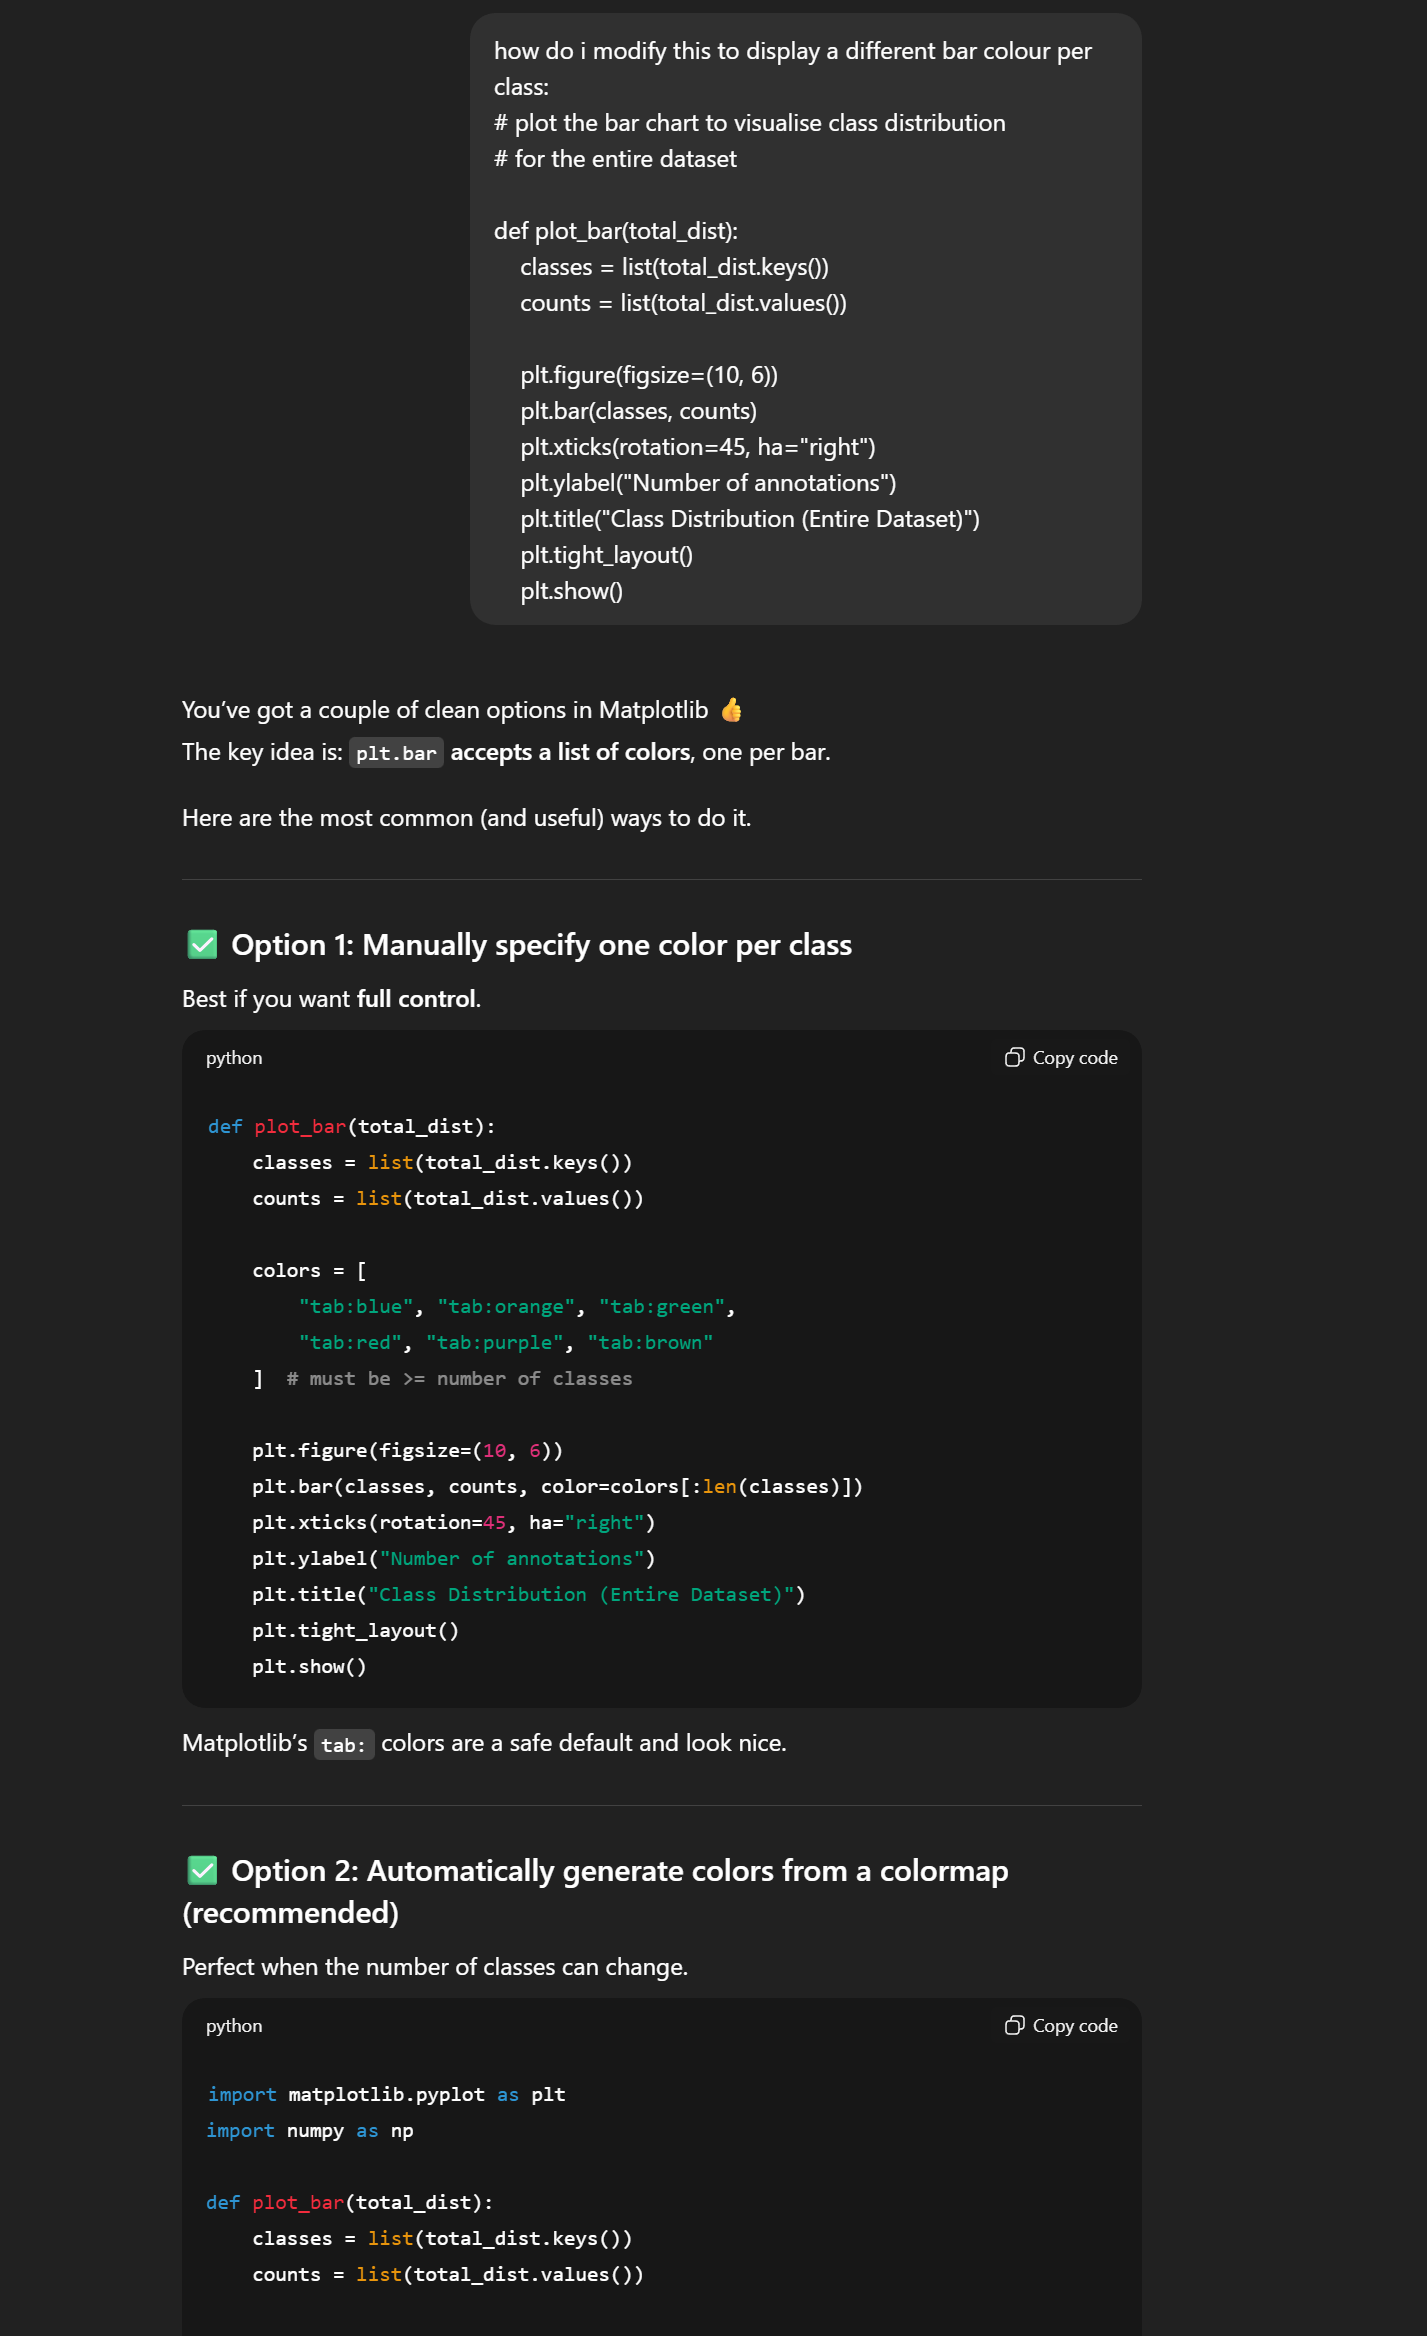
\includegraphics[width=\textwidth]{code1.png}
    \end{subfigure}
    \hfill
    \begin{subfigure}[b]{0.45\textwidth}
        \centering
        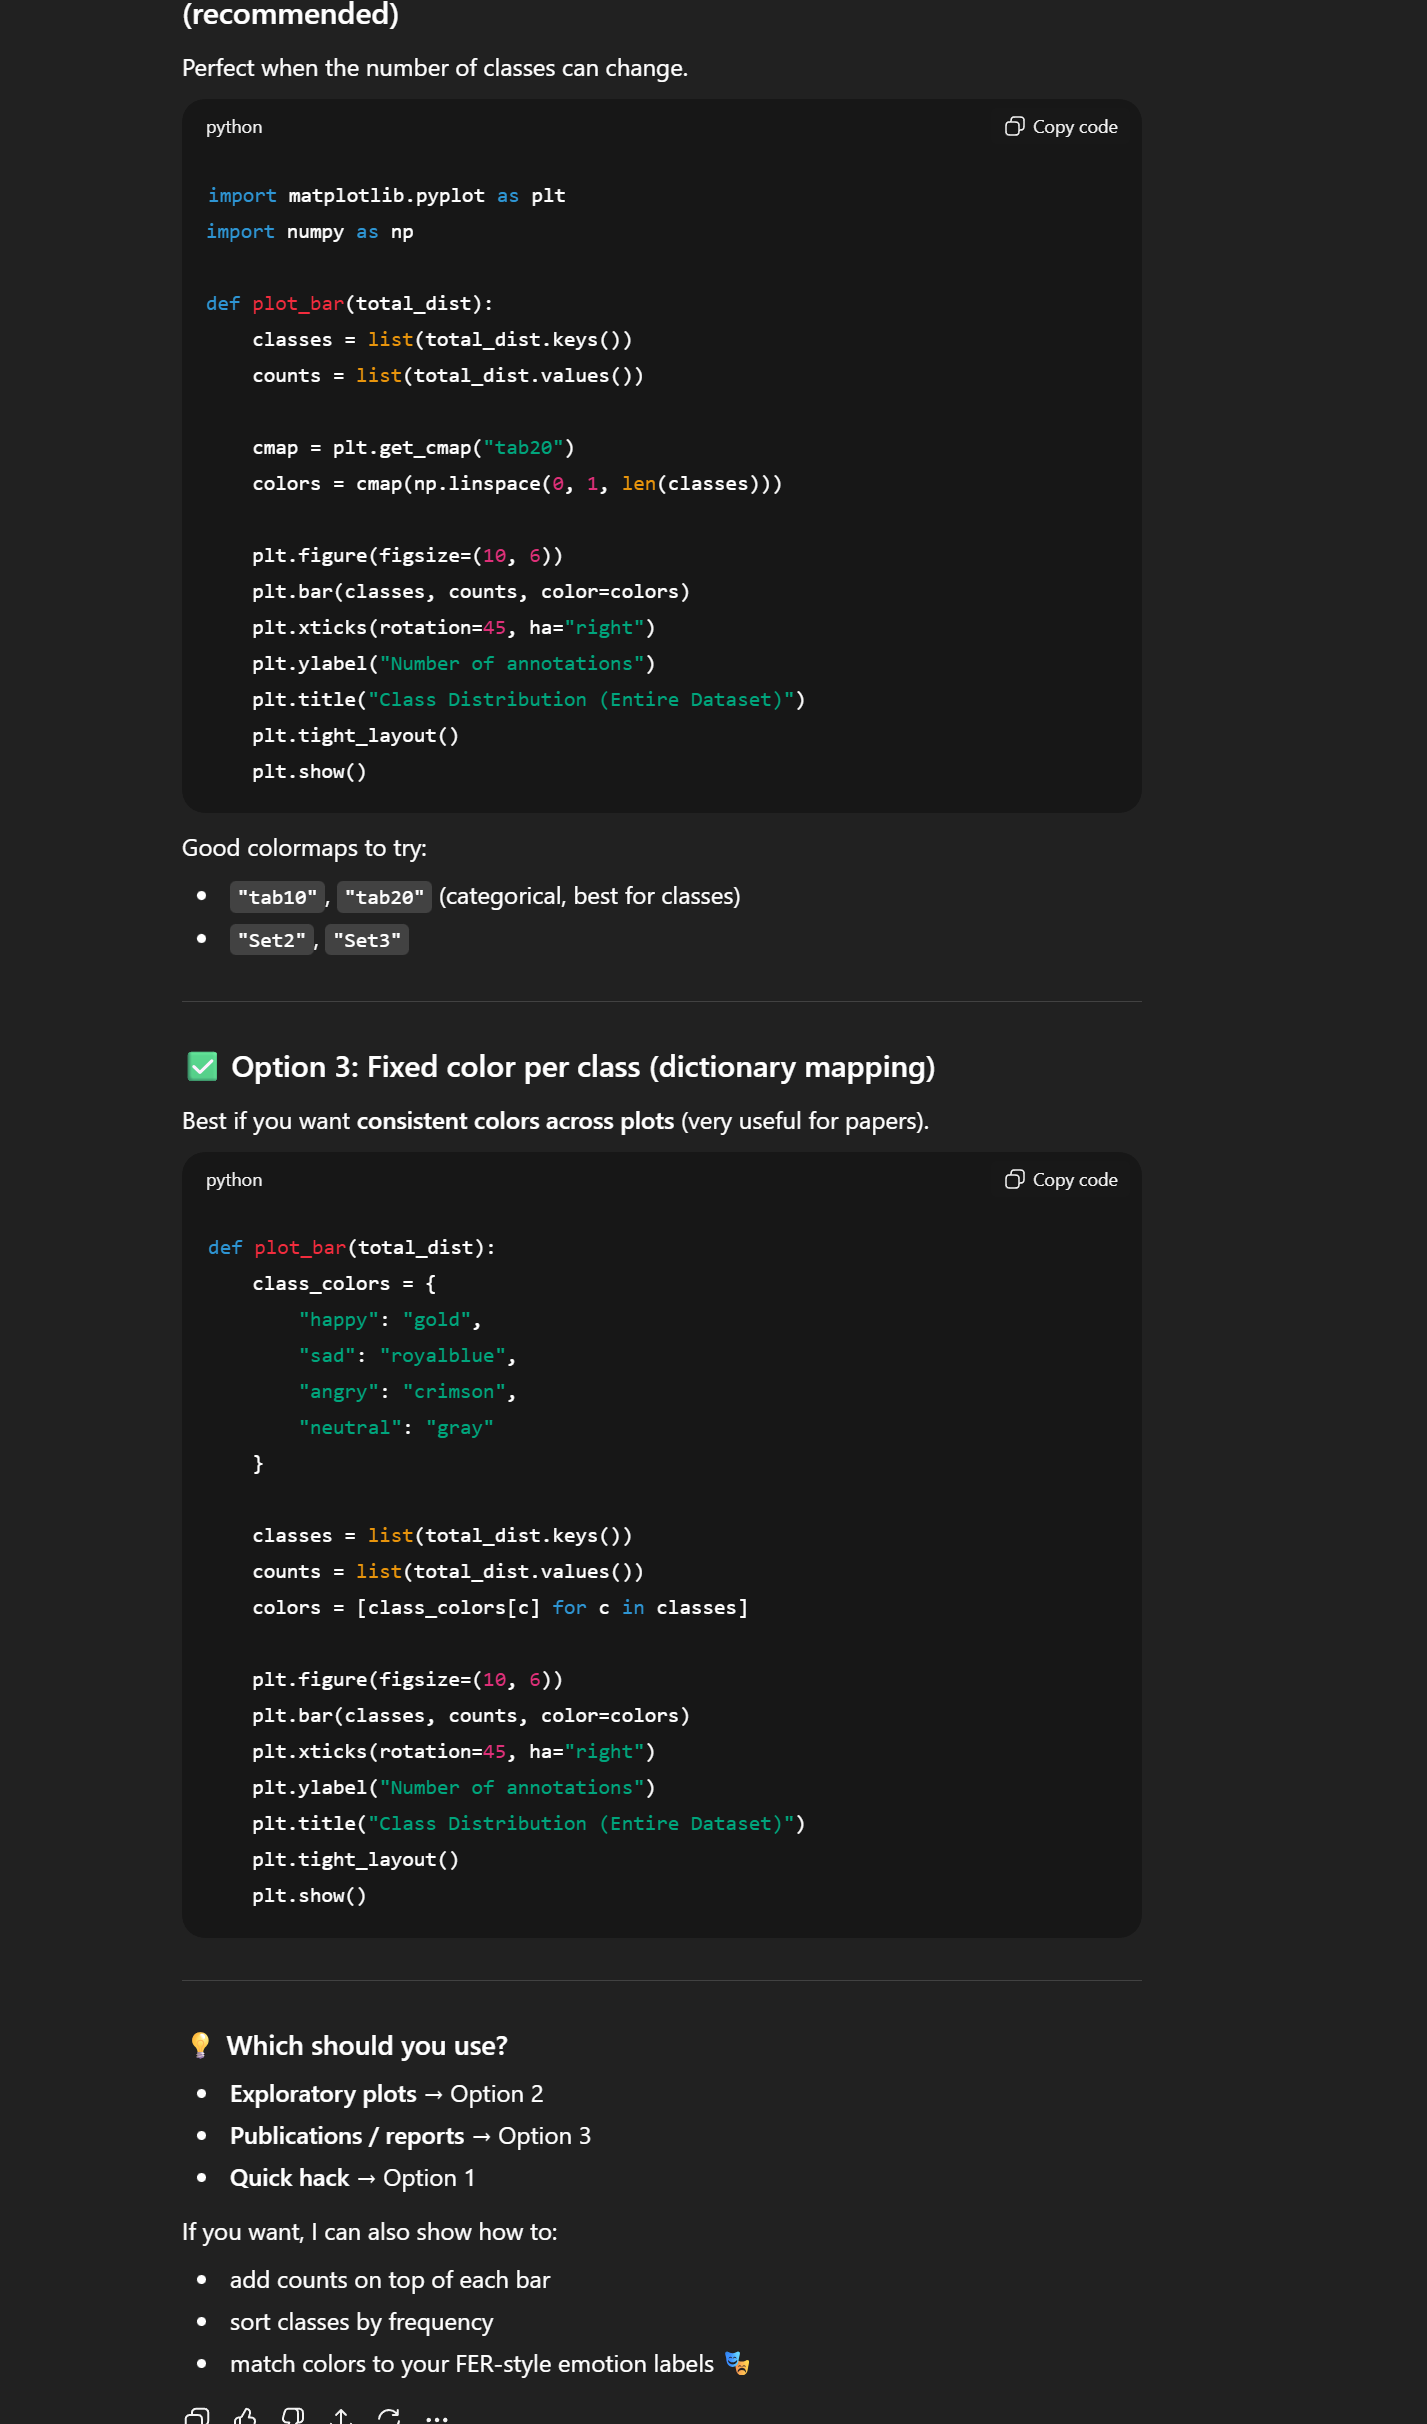
\includegraphics[width=\textwidth]{code2.png}
    \end{subfigure}
    \caption{Prompt: Asking for code suggestions}\label{fig:code}
\end{figure}

Not all code suggestions given by the AI tools was useful, which is why the output was not just copied but was carefully reviewed and tested before being integrated to ensure that it does what is intended, and to ensure that we understood what the code was actually doing.

\subsubsection*{Literature Review help}

NotebookLM was used as a tool to help with the process of writing the Background for the report. It was used to provide summaries of the core concepts in the papers relevant to the object detectors we were researching, helping gain a better understanding of the content in the paper, as shown in Figure~\ref{fig:litreview}. This was useful as it made new concepts simpler to understand by providing concise points of the main content in the papers.

\begin{figure}[htbp]
    \centering
    \begin{subfigure}[b]{0.46\textwidth}
        \centering
        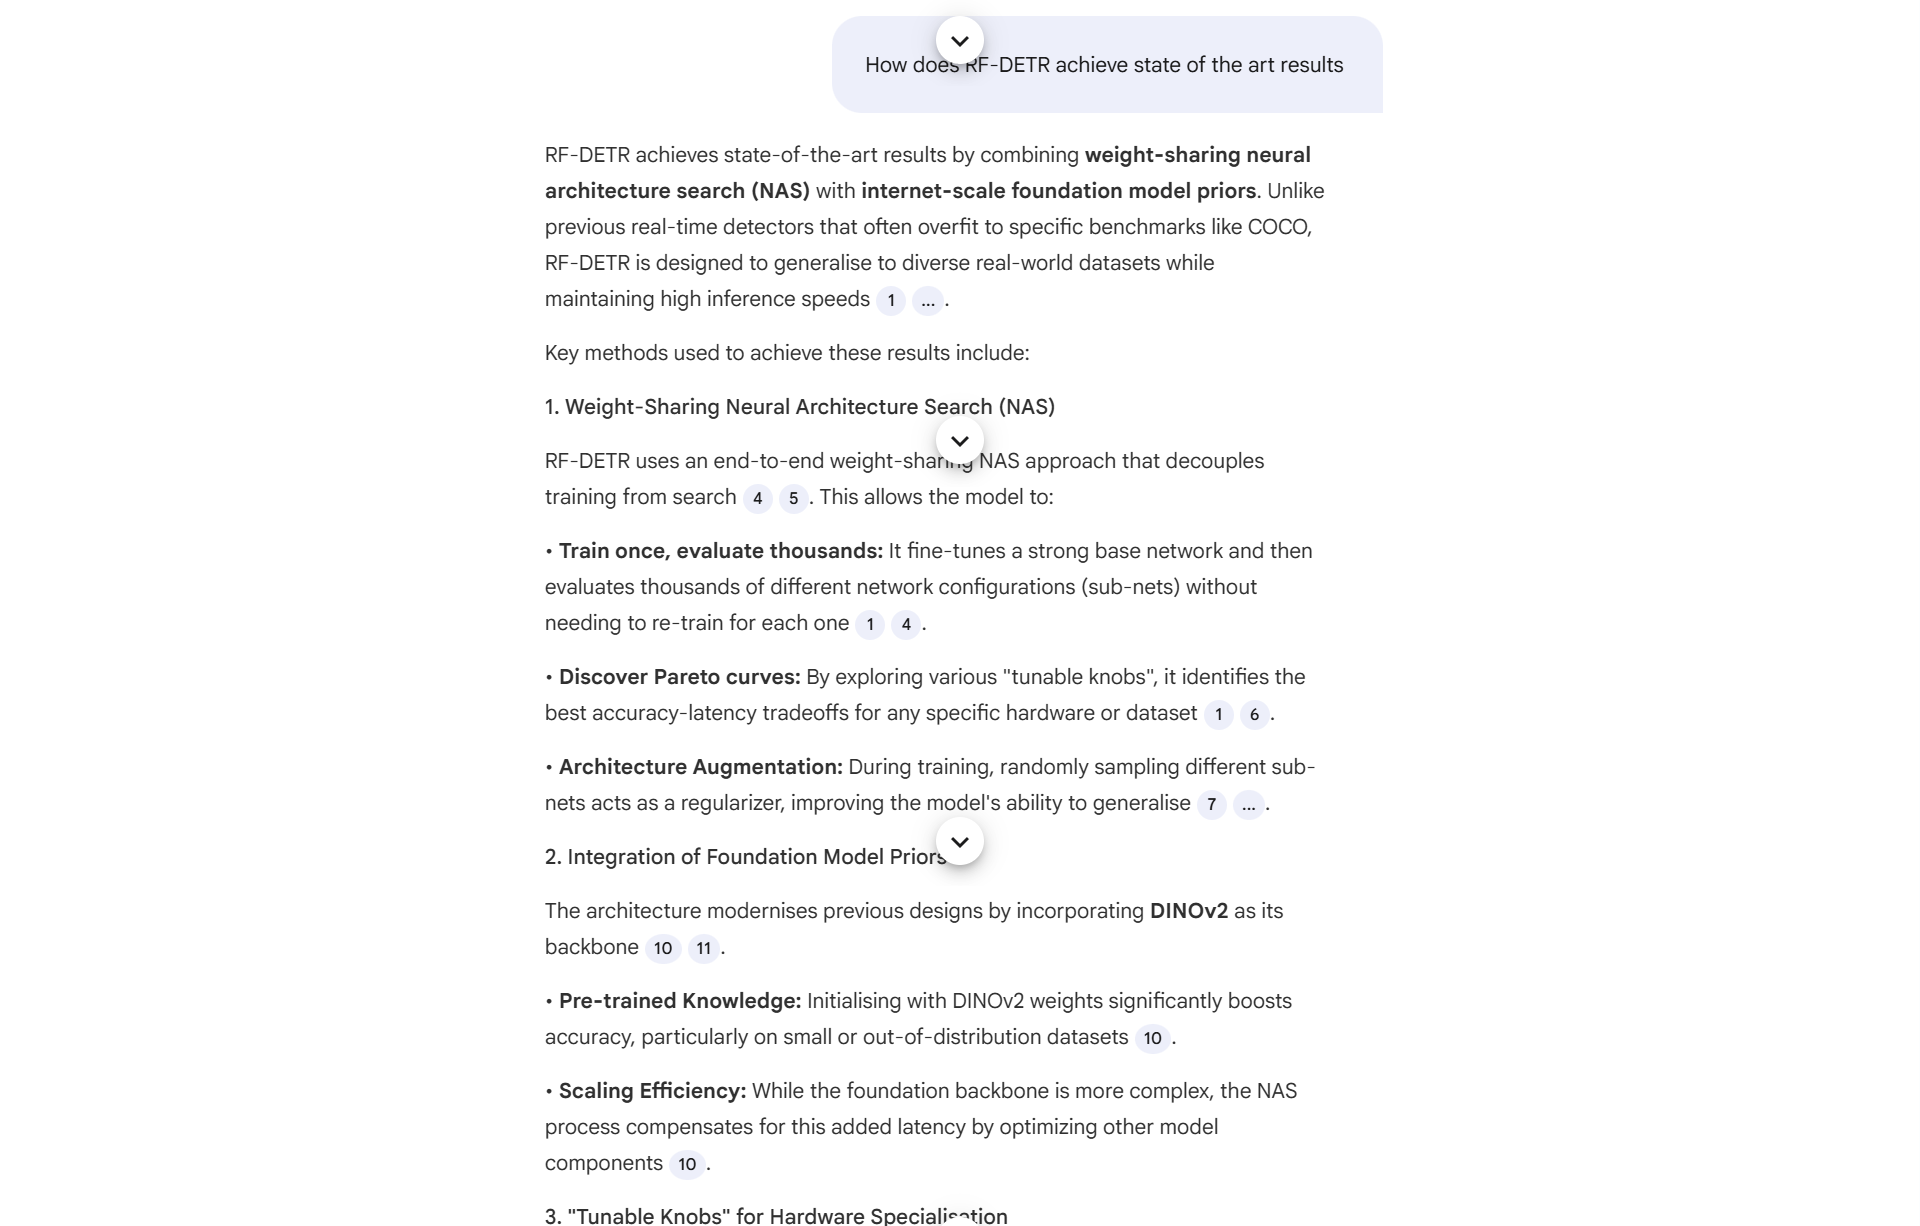
\includegraphics[width=\textwidth]{litreview1.png}
    \end{subfigure}
    \hfill
    \begin{subfigure}[b]{0.46\textwidth}
        \centering
        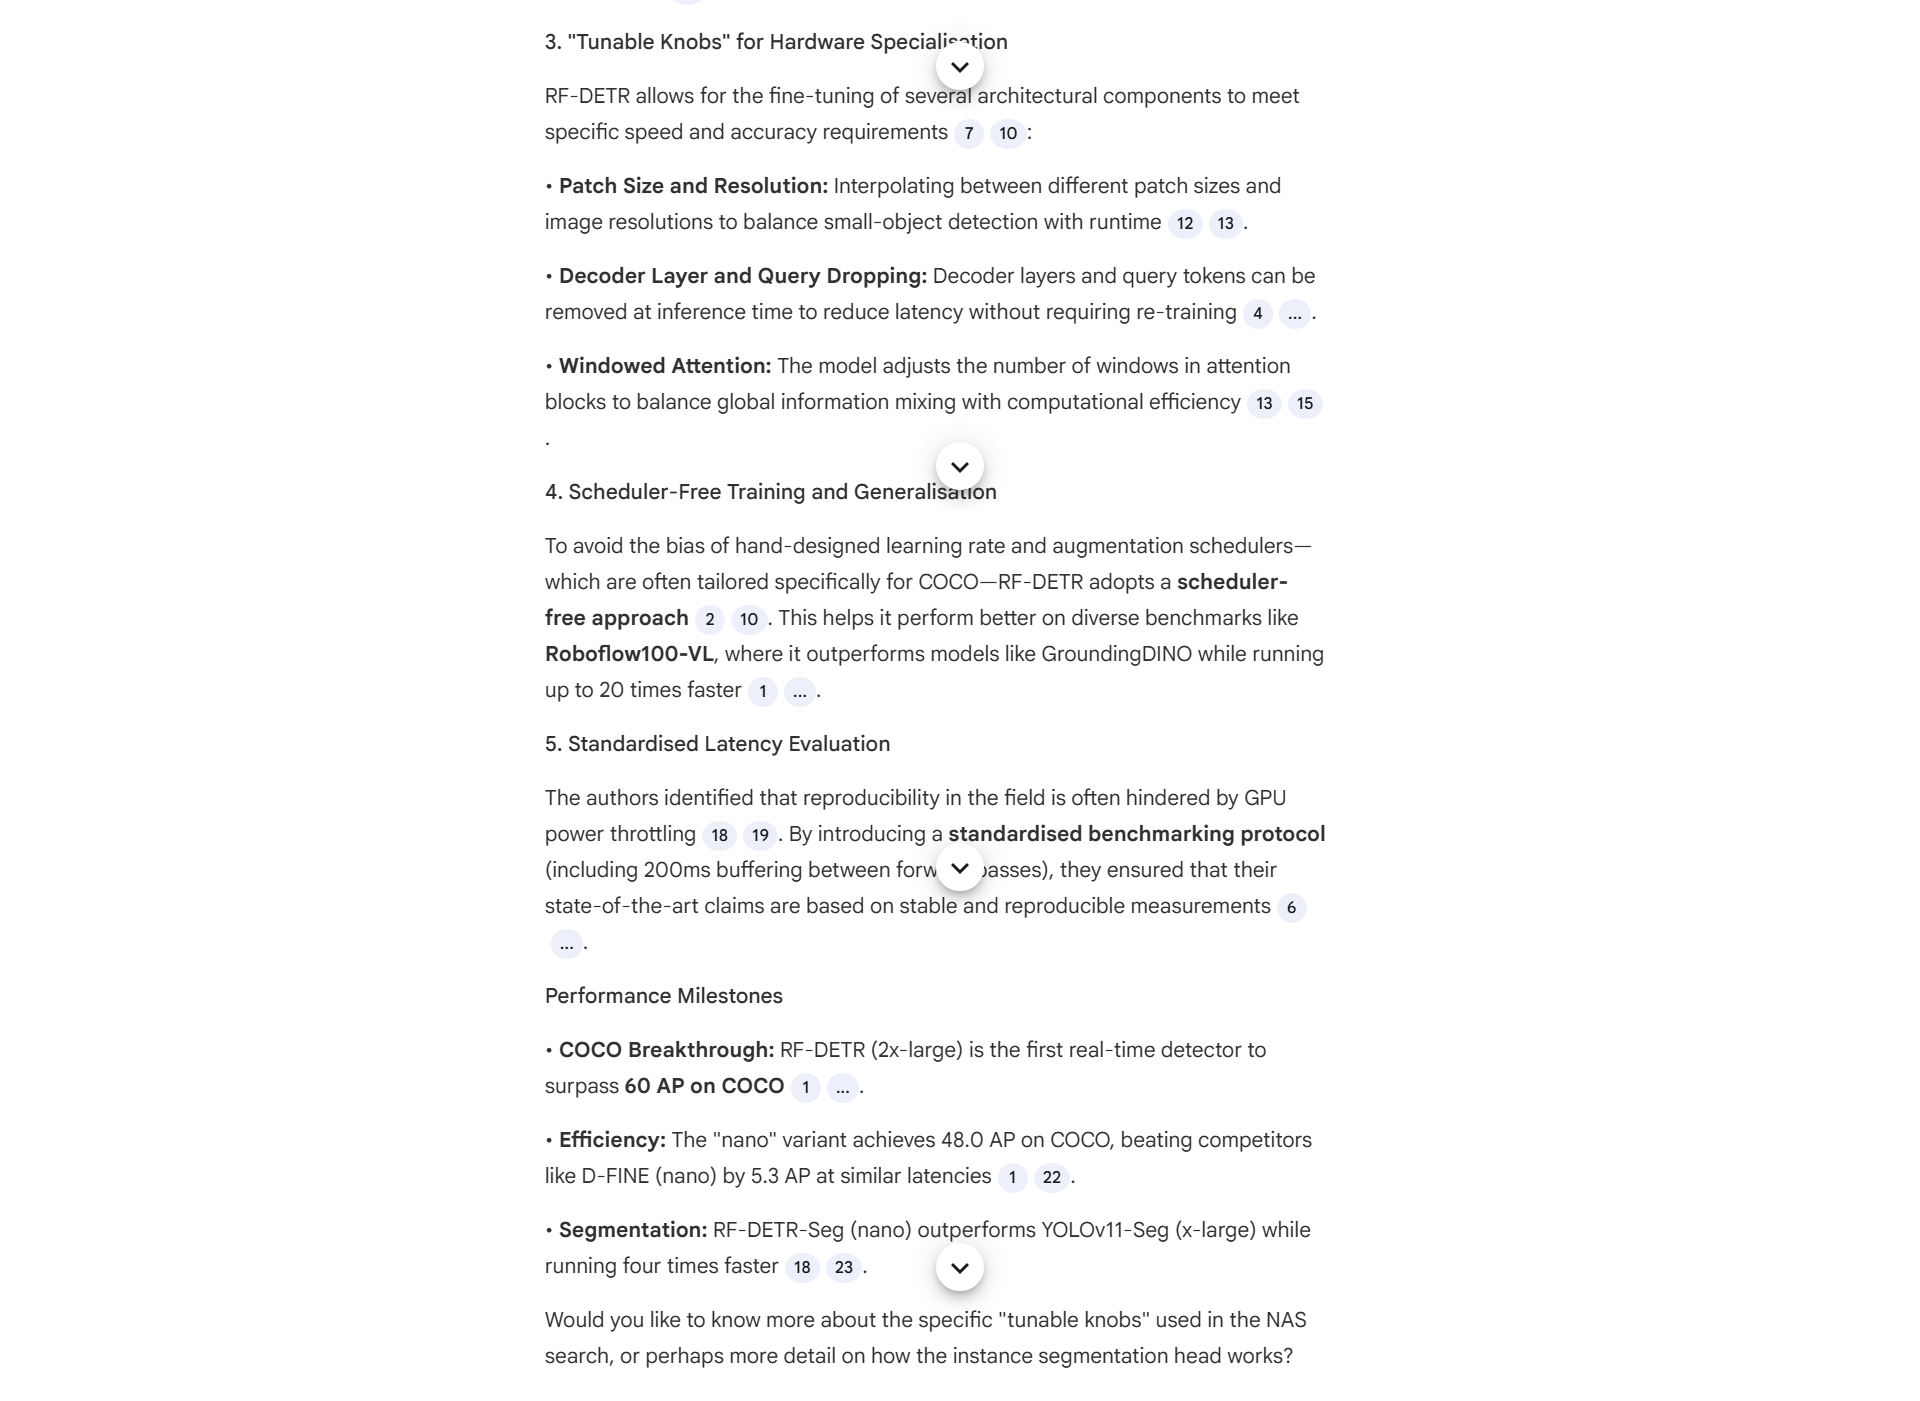
\includegraphics[width=\textwidth]{litreview2.png}
    \end{subfigure}
    \caption{Prompt: Summarizing a paper}\label{fig:litreview}
\end{figure}

After going through the points and explanations given by NotebookLM, the output was verified by reading through the relevant parts of the actual paper itself. This ensured we gained an accurate understanding of the actual content

\section{Improvements, Errors and Contributions}
% Discuss the areas where generative AI contributed to enhancing your work or instances where the output contained errors. This can include but is not limited to, data analysis, formulation of ethical considerations, literature review enhancement, or idea generation. Highlight specific cases where this happened.
Generative AI tools significantly enhanced our efficiency in most aspects of this project. The ability to quickly suggest relevant code snippets, debug issues, and generate documentation outlines allowed us to focus more on higher-level problem-solving and less on routine tasks. However, it was crucial to maintain a critical eye on the AI-generated content, as not all suggestions were accurate or contextually appropriate. This experience has reinforced the importance of human oversight in AI-assisted workflows. Overall, the integration of generative AI has positively influenced our approach to academic projects, highlighting both its potential and limitations.

In particular, generative AI provided assistance in finding relevant library documentation and usage examples, deepening our understanding of the tools we used. It also helped in brainstorming solutions for complex problems, offering alternative perspectives that we might not have considered otherwise. From our experience, the smaller, free versions of these models struggled with understanding the code, as the structure of jupyter notebooks often either `confuses' the model or perhaps it does not fit in the context window properly. This led to some frustrating experiences where the model would provide irrelevant or incorrect suggestions. However, when using the more advanced models with larger context windows, we found that they were better able to understand the code structure and provide more accurate suggestions.

Aside from code-related tasks, generative AI also contributed to the formulation of the documentation by providing structured outlines and suggestions for content organization. This was helpful in ensuring that the report was well structured, as well as aiding us in splitting up the work among team members, ensuring more-or-less equal contributions.

\section{Individual Reflection}
% Reflect on your personal experience using generative AI in your project. Discuss what you learned, what surprised you, and how your perspective on using AI in academic projects has changed, if at all. Did Gen AI help you be more efficient? Do you feel you wasted more time when you used it? For which part was it most helpful? Literature review, debugging?
Generative AI has become a widely adopted tool in various fields, including academic research and project development. Thus, as students, we believe that it is necessary to make use of these tools in order to better understand their capabilities and limitations.

From a personal perspective, over the 3 years of this degree, We have seen a significant evolution in the capabilities of generative AI tools. Initially, these tools were limited in their ability to understand context and provide relevant suggestions, and would most certainly have struggled to assist with this project. However, advancements in the relevant fields have resulted in more sophisticated models that can comprehend complex code structures and provide meaningful assistance. We've realized that, despite the significant improvements in the tools since we first encountered them, they are still able to make mistakes, and thus our trust in them has not increased significantly. We have learned to approach AI-generated content with a critical mindset, verifying its accuracy and relevance before integration.


\newpage\pagenumbering{roman}
\section{References and List of Resources Used}
% List references or resources consulted about generative AI.

\begin{thebibliography}{99}

    \bibitem{gemini}
    Google, ``Gemini 3 Pro,'' Nov. 2025. [Online]. Available: \url{https://gemini.google.com/}

    \bibitem{claude}
    Anthropic, ``Claude Sonnet 4.5,'' Sep. 2025. [Online]. Available: \url{https://claude.ai/}

    \bibitem{chatgpt}
    OpenAI, ``ChatGPT (GPT-5.2),'' Dec. 2025. [Online]. Available: \url{https://chatgpt.com/}


    \bibitem{antigravity}
    Google DeepMind, ``Antigravity: Advanced Agentic Coding Assistant,'' 2026. [Online].

    \bibitem{notebooklm}
    Google, ``NotebookLM,'' \textit{Google Labs}, 2023. [Online]. Available: \url{https://notebooklm.google.com/}
\end{thebibliography}


\end{document}
